% Tiago Tresoldi presentation

\documentclass{beamer}

\usepackage{graphicx}

\usepackage{./beamerthemempiis}

\usepackage{colortbl}

\usepackage{tipa}

\usepackage{hyperref}

\usepackage{amssymb}
\let\oldemptyset\emptyset
\let\emptyset\varnothing

\begin{document}
\title{QMSS16 Presentation: \\ Distinct Phonetic Features for Language Phylogeny}   
\author{Tiago Tresoldi} 
\date{May 18\textsuperscript{th}, 2016} 


\frame{\titlepage} 


\section{The questions and the problems} 
\frame{\frametitle{The questions and the problems}
\begin{itemize}
\item Is it possible (and useful) to use phonology in language phylogeny?
	\begin{itemize}
	\item Phonology has a high rate of evolution, but borrowing is rare
	\item Diachronic and synchronic data for estimation of transition probabilities
	\end{itemize}
\item Hypothesis: language philogeny using distinct features (``the most basic unit of analysis in
      phonetic structures''), adapted from Jakobson \textit{et al.} (1941--1956),
	  Chomsky \&{} Halle (1968--1983), and, in particular, Ladefoged (1971; 1993)
	\begin{itemize}
	\item Pros: binary (and mostly non-exclusive) features (no dummy variables!),
	      single model for vowels and consonants
	\item Traditional reconstruction (such as for the IE family) uses words mostly as proxy
	      for phonology, but we should combine lexical and phonological data
	\end{itemize}
\end{itemize} 
}



\frame{\frametitle{The data}

\begin{table}[]
\centering
\caption{Phonetic reflexes (snippet)}
\label{table-phonemes}
\begin{tabular}{lllllll}
PIE & O. Irish & Latin & O. English & Lith. & Toch. B & Arm. \\
*p   & $\emptyset$         & p     & f           & p     & p  & h   \\
*\'{g}\textsuperscript{h}i & g         & h     & g           & \textipa{Z}   & \textipa{C}    & \textdzlig   \\
*k\textsuperscript{w}  & k         & k\textsuperscript{w}    & h\textsuperscript{w}          & k & k   & k\textsuperscript{h}     
\end{tabular}
\end{table}

\begin{table}[]
\centering
\caption{Distinct features of phonetic reflexes (snippet)}
\label{table-reflexes}
\begin{tabular}{llllllll}
            & p.ant & p.obstr & p.lab & \'{g}\textsuperscript{h}i.obstr & \'{g}\textsuperscript{h}i.cor \\
Old Irish   & -     & -       & -     & T       & F           \\
Latin       & F     & T       & T     & T       & F           \\
Old English & T     & T       & F     & T       & F           \\
Lithuanian  & F     & T       & T     & T       & T          
\end{tabular}
\end{table}

}

\section{The (very, very first) results}
\frame{\frametitle{The (very, very first) results}
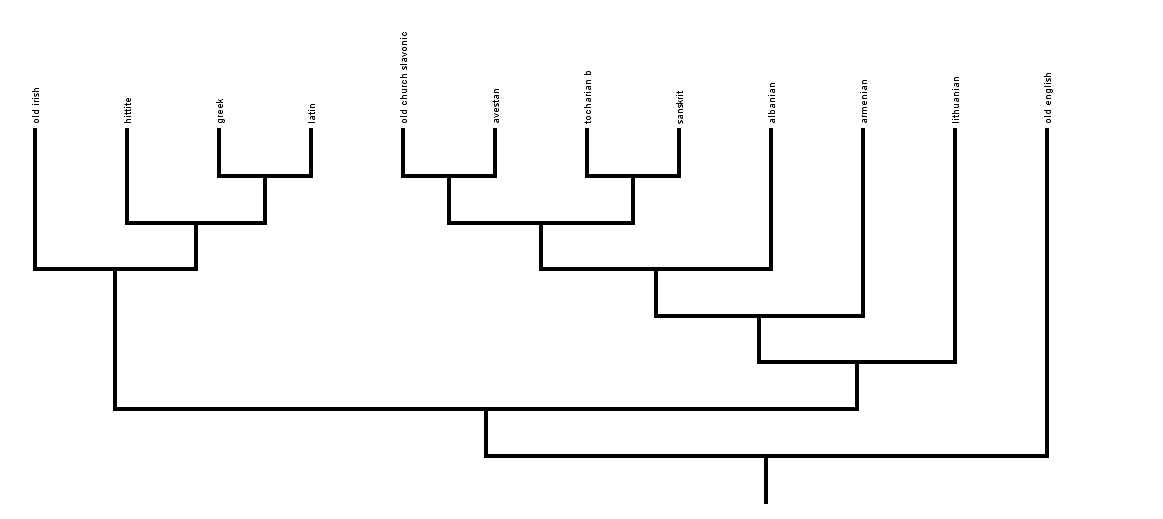
\includegraphics[scale=0.41]{tree.png}
}

\section{Final words} 
\frame{\frametitle{Final words}
\begin{itemize}
\item Without constrains and additional data, the tree is
      mirroring similarities in phoneme inventories, not language history

\item Ancestral State Recostruction -- do results from traditional methods match those
      of phylogenetic ones?
\begin{itemize}
	\item Data from MPI banks (PHOIBLE, ``Intercontinental Dictionary Series''),
	      paper dictionaries (and web scraping...)
	\item Tools: phylogenetic software, \texttt{lingpy}
	\item Combine known data and phylogeny to infer best model and the order of ancestral state changes
\end{itemize}

\item Code on GitHub (\url{https://github.com/tresoldi/qmss2016})

\item Some bold, dreamy research questions:
	\begin{itemize}
	\item How confident can we be on the presence of laryngeals in PIE? What is the most likely
	      date for their evolution? What were they most likely values? How many there were?
		  (quantitative criticism of Voyles \&{} Barrack, 2015)
	\item How confident can we be of Etruscan as a colonial Luwian language? (cf. Woudhuizen, 2008)
	\end{itemize}
\end{itemize} 
}

\end{document}